Fig.~\ref{fig:prefetcher_speedup} shows the speedup of our best prefetcher
compared to running the test without a prefetcher. As you can see from the
chart there is an all-round good speedup, in addition to certain test which
have higher speedup. Only the \emph{twolf} benchmark runs slower with the
prefetcher.

\begin{figure}
	% GNUPLOT: LaTeX picture with Postscript
\begingroup
  \makeatletter
  \providecommand\color[2][]{%
    \GenericError{(gnuplot) \space\space\space\@spaces}{%
      Package color not loaded in conjunction with
      terminal option `colourtext'%
    }{See the gnuplot documentation for explanation.%
    }{Either use 'blacktext' in gnuplot or load the package
      color.sty in LaTeX.}%
    \renewcommand\color[2][]{}%
  }%
  \providecommand\includegraphics[2][]{%
    \GenericError{(gnuplot) \space\space\space\@spaces}{%
      Package graphicx or graphics not loaded%
    }{See the gnuplot documentation for explanation.%
    }{The gnuplot epslatex terminal needs graphicx.sty or graphics.sty.}%
    \renewcommand\includegraphics[2][]{}%
  }%
  \providecommand\rotatebox[2]{#2}%
  \@ifundefined{ifGPcolor}{%
    \newif\ifGPcolor
    \GPcolortrue
  }{}%
  \@ifundefined{ifGPblacktext}{%
    \newif\ifGPblacktext
    \GPblacktexttrue
  }{}%
  % define a \g@addto@macro without @ in the name:
  \let\gplgaddtomacro\g@addto@macro
  % define empty templates for all commands taking text:
  \gdef\gplbacktext{}%
  \gdef\gplfronttext{}%
  \makeatother
  \ifGPblacktext
    % no textcolor at all
    \def\colorrgb#1{}%
    \def\colorgray#1{}%
  \else
    % gray or color?
    \ifGPcolor
      \def\colorrgb#1{\color[rgb]{#1}}%
      \def\colorgray#1{\color[gray]{#1}}%
      \expandafter\def\csname LTw\endcsname{\color{white}}%
      \expandafter\def\csname LTb\endcsname{\color{black}}%
      \expandafter\def\csname LTa\endcsname{\color{black}}%
      \expandafter\def\csname LT0\endcsname{\color[rgb]{1,0,0}}%
      \expandafter\def\csname LT1\endcsname{\color[rgb]{0,1,0}}%
      \expandafter\def\csname LT2\endcsname{\color[rgb]{0,0,1}}%
      \expandafter\def\csname LT3\endcsname{\color[rgb]{1,0,1}}%
      \expandafter\def\csname LT4\endcsname{\color[rgb]{0,1,1}}%
      \expandafter\def\csname LT5\endcsname{\color[rgb]{1,1,0}}%
      \expandafter\def\csname LT6\endcsname{\color[rgb]{0,0,0}}%
      \expandafter\def\csname LT7\endcsname{\color[rgb]{1,0.3,0}}%
      \expandafter\def\csname LT8\endcsname{\color[rgb]{0.5,0.5,0.5}}%
    \else
      % gray
      \def\colorrgb#1{\color{black}}%
      \def\colorgray#1{\color[gray]{#1}}%
      \expandafter\def\csname LTw\endcsname{\color{white}}%
      \expandafter\def\csname LTb\endcsname{\color{black}}%
      \expandafter\def\csname LTa\endcsname{\color{black}}%
      \expandafter\def\csname LT0\endcsname{\color{black}}%
      \expandafter\def\csname LT1\endcsname{\color{black}}%
      \expandafter\def\csname LT2\endcsname{\color{black}}%
      \expandafter\def\csname LT3\endcsname{\color{black}}%
      \expandafter\def\csname LT4\endcsname{\color{black}}%
      \expandafter\def\csname LT5\endcsname{\color{black}}%
      \expandafter\def\csname LT6\endcsname{\color{black}}%
      \expandafter\def\csname LT7\endcsname{\color{black}}%
      \expandafter\def\csname LT8\endcsname{\color{black}}%
    \fi
  \fi
  \setlength{\unitlength}{0.0500bp}%
  \begin{picture}(5100.00,5100.00)%
    \gplgaddtomacro\gplbacktext{%
      \csname LTb\endcsname%
      \put(561,654){\makebox(0,0)[r]{\strut{} 0.8}}%
      \put(561,1502){\makebox(0,0)[r]{\strut{} 1}}%
      \put(561,2350){\makebox(0,0)[r]{\strut{} 1.2}}%
      \put(561,3199){\makebox(0,0)[r]{\strut{} 1.4}}%
      \put(561,4047){\makebox(0,0)[r]{\strut{} 1.6}}%
      \put(561,4895){\makebox(0,0)[r]{\strut{} 1.8}}%
      \put(981,552){\rotatebox{-45}{\makebox(0,0)[l]{\strut{}ammp}}}%
      \put(1298,552){\rotatebox{-45}{\makebox(0,0)[l]{\strut{}applu}}}%
      \put(1616,552){\rotatebox{-45}{\makebox(0,0)[l]{\strut{}apsi}}}%
      \put(1934,552){\rotatebox{-45}{\makebox(0,0)[l]{\strut{}art110}}}%
      \put(2251,552){\rotatebox{-45}{\makebox(0,0)[l]{\strut{}art470}}}%
      \put(2569,552){\rotatebox{-45}{\makebox(0,0)[l]{\strut{}bzip2 graphic}}}%
      \put(2887,552){\rotatebox{-45}{\makebox(0,0)[l]{\strut{}bzip2 program}}}%
      \put(3205,552){\rotatebox{-45}{\makebox(0,0)[l]{\strut{}bzip2 source}}}%
      \put(3522,552){\rotatebox{-45}{\makebox(0,0)[l]{\strut{}galgel}}}%
      \put(3840,552){\rotatebox{-45}{\makebox(0,0)[l]{\strut{}swim}}}%
      \put(4158,552){\rotatebox{-45}{\makebox(0,0)[l]{\strut{}twolf}}}%
      \put(4475,552){\rotatebox{-45}{\makebox(0,0)[l]{\strut{}wupwise}}}%
    }%
    \gplgaddtomacro\gplfronttext{%
      \csname LTb\endcsname%
      \put(4005,4728){\makebox(0,0)[r]{\strut{}RPT}}%
      \csname LTb\endcsname%
      \put(4005,4542){\makebox(0,0)[r]{\strut{}DCPT}}%
      \csname LTb\endcsname%
      \put(4005,4356){\makebox(0,0)[r]{\strut{}Our prefetcher}}%
      \csname LTb\endcsname%
      \put(4005,4170){\makebox(0,0)[r]{\strut{}No prefetcher}}%
    }%
    \gplbacktext
    \put(0,0){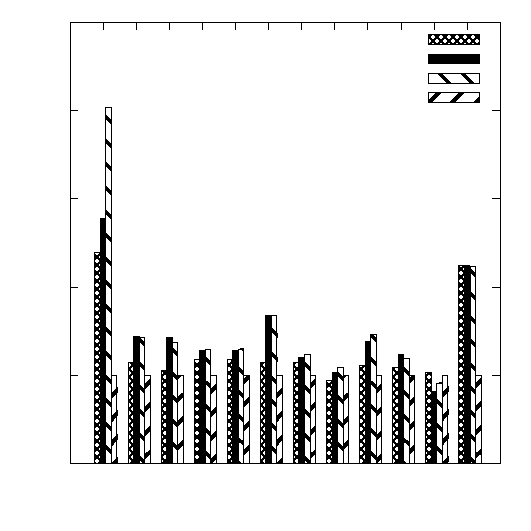
\includegraphics{spec}}%
    \gplfronttext
  \end{picture}%
\endgroup

	\caption{Prefetcher speedup chart}
	\label{fig:prefetcher_speedup}
\end{figure}

\subsection{Table Parameters}
Fig.~\ref{fig:table_size_chart} shows the speedup with different table sizes.
%As you can see from Fig.~\ref{fig:table_size_chart}, the performance stopped
%increasing after a table size of 256. This we believe is caused by instruction
%conflicts in the table. When the table reaches a certain size, most
%instructions get their own place in the table, and avoid being evicted by
%conflicting instructions.

\begin{figure}
	% GNUPLOT: LaTeX picture with Postscript
\begingroup
  \makeatletter
  \providecommand\color[2][]{%
    \GenericError{(gnuplot) \space\space\space\@spaces}{%
      Package color not loaded in conjunction with
      terminal option `colourtext'%
    }{See the gnuplot documentation for explanation.%
    }{Either use 'blacktext' in gnuplot or load the package
      color.sty in LaTeX.}%
    \renewcommand\color[2][]{}%
  }%
  \providecommand\includegraphics[2][]{%
    \GenericError{(gnuplot) \space\space\space\@spaces}{%
      Package graphicx or graphics not loaded%
    }{See the gnuplot documentation for explanation.%
    }{The gnuplot epslatex terminal needs graphicx.sty or graphics.sty.}%
    \renewcommand\includegraphics[2][]{}%
  }%
  \providecommand\rotatebox[2]{#2}%
  \@ifundefined{ifGPcolor}{%
    \newif\ifGPcolor
    \GPcolortrue
  }{}%
  \@ifundefined{ifGPblacktext}{%
    \newif\ifGPblacktext
    \GPblacktexttrue
  }{}%
  % define a \g@addto@macro without @ in the name:
  \let\gplgaddtomacro\g@addto@macro
  % define empty templates for all commands taking text:
  \gdef\gplbacktext{}%
  \gdef\gplfronttext{}%
  \makeatother
  \ifGPblacktext
    % no textcolor at all
    \def\colorrgb#1{}%
    \def\colorgray#1{}%
  \else
    % gray or color?
    \ifGPcolor
      \def\colorrgb#1{\color[rgb]{#1}}%
      \def\colorgray#1{\color[gray]{#1}}%
      \expandafter\def\csname LTw\endcsname{\color{white}}%
      \expandafter\def\csname LTb\endcsname{\color{black}}%
      \expandafter\def\csname LTa\endcsname{\color{black}}%
      \expandafter\def\csname LT0\endcsname{\color[rgb]{1,0,0}}%
      \expandafter\def\csname LT1\endcsname{\color[rgb]{0,1,0}}%
      \expandafter\def\csname LT2\endcsname{\color[rgb]{0,0,1}}%
      \expandafter\def\csname LT3\endcsname{\color[rgb]{1,0,1}}%
      \expandafter\def\csname LT4\endcsname{\color[rgb]{0,1,1}}%
      \expandafter\def\csname LT5\endcsname{\color[rgb]{1,1,0}}%
      \expandafter\def\csname LT6\endcsname{\color[rgb]{0,0,0}}%
      \expandafter\def\csname LT7\endcsname{\color[rgb]{1,0.3,0}}%
      \expandafter\def\csname LT8\endcsname{\color[rgb]{0.5,0.5,0.5}}%
    \else
      % gray
      \def\colorrgb#1{\color{black}}%
      \def\colorgray#1{\color[gray]{#1}}%
      \expandafter\def\csname LTw\endcsname{\color{white}}%
      \expandafter\def\csname LTb\endcsname{\color{black}}%
      \expandafter\def\csname LTa\endcsname{\color{black}}%
      \expandafter\def\csname LT0\endcsname{\color{black}}%
      \expandafter\def\csname LT1\endcsname{\color{black}}%
      \expandafter\def\csname LT2\endcsname{\color{black}}%
      \expandafter\def\csname LT3\endcsname{\color{black}}%
      \expandafter\def\csname LT4\endcsname{\color{black}}%
      \expandafter\def\csname LT5\endcsname{\color{black}}%
      \expandafter\def\csname LT6\endcsname{\color{black}}%
      \expandafter\def\csname LT7\endcsname{\color{black}}%
      \expandafter\def\csname LT8\endcsname{\color{black}}%
    \fi
  \fi
  \setlength{\unitlength}{0.0500bp}%
  \begin{picture}(5100.00,5100.00)%
    \gplgaddtomacro\gplbacktext{%
      \csname LTb\endcsname%
      \put(663,372){\makebox(0,0)[r]{\strut{} 1.03}}%
      \put(663,937){\makebox(0,0)[r]{\strut{} 1.04}}%
      \put(663,1503){\makebox(0,0)[r]{\strut{} 1.05}}%
      \put(663,2068){\makebox(0,0)[r]{\strut{} 1.06}}%
      \put(663,2634){\makebox(0,0)[r]{\strut{} 1.07}}%
      \put(663,3199){\makebox(0,0)[r]{\strut{} 1.08}}%
      \put(663,3764){\makebox(0,0)[r]{\strut{} 1.09}}%
      \put(663,4330){\makebox(0,0)[r]{\strut{} 1.1}}%
      \put(663,4895){\makebox(0,0)[r]{\strut{} 1.11}}%
      \put(765,186){\makebox(0,0){\strut{} 16}}%
      \put(1213,186){\makebox(0,0){\strut{} 32}}%
      \put(1660,186){\makebox(0,0){\strut{} 64}}%
      \put(2108,186){\makebox(0,0){\strut{} 128}}%
      \put(2555,186){\makebox(0,0){\strut{} 256}}%
      \put(3003,186){\makebox(0,0){\strut{} 512}}%
      \put(3450,186){\makebox(0,0){\strut{} 1024}}%
      \put(3898,186){\makebox(0,0){\strut{} 2048}}%
      \put(4345,186){\makebox(0,0){\strut{} 4096}}%
      \put(4793,186){\makebox(0,0){\strut{} 8192}}%
    }%
    \gplgaddtomacro\gplfronttext{%
    }%
    \gplbacktext
    \put(0,0){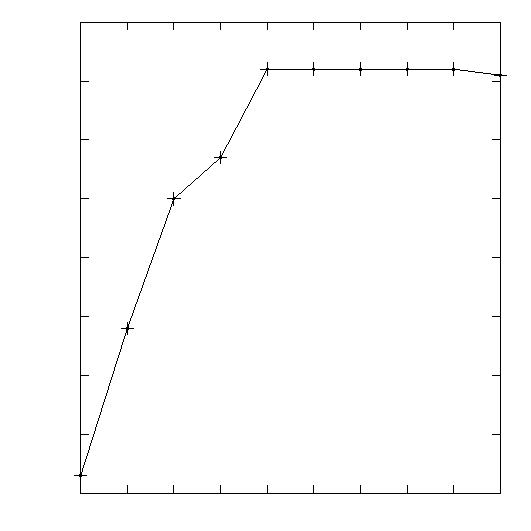
\includegraphics{tablesize}}%
    \gplfronttext
  \end{picture}%
\endgroup

	\caption{Speedup with different table sizes}
	\label{fig:table_size_chart}
\end{figure}

\subsection{Most Common Stride Parameters}

The final solution was selected after thorough testing and tweaking of the
prefetcher. The different results from the tests can be seen in
Fig.~\ref{fig:prefetcher_tweaks}. Each line represents different values for the
threshold, and the x-axis shows the values for the count variable. From the
figure we can clearly see which parameters provides the best speedup. The
figure also showed the line for threshold 4 rising at the end of the chart,
which is the reason for the additional data point aquired by running a single
extra test.

\begin{figure}
	% GNUPLOT: LaTeX picture with Postscript
\begingroup
  \makeatletter
  \providecommand\color[2][]{%
    \GenericError{(gnuplot) \space\space\space\@spaces}{%
      Package color not loaded in conjunction with
      terminal option `colourtext'%
    }{See the gnuplot documentation for explanation.%
    }{Either use 'blacktext' in gnuplot or load the package
      color.sty in LaTeX.}%
    \renewcommand\color[2][]{}%
  }%
  \providecommand\includegraphics[2][]{%
    \GenericError{(gnuplot) \space\space\space\@spaces}{%
      Package graphicx or graphics not loaded%
    }{See the gnuplot documentation for explanation.%
    }{The gnuplot epslatex terminal needs graphicx.sty or graphics.sty.}%
    \renewcommand\includegraphics[2][]{}%
  }%
  \providecommand\rotatebox[2]{#2}%
  \@ifundefined{ifGPcolor}{%
    \newif\ifGPcolor
    \GPcolortrue
  }{}%
  \@ifundefined{ifGPblacktext}{%
    \newif\ifGPblacktext
    \GPblacktexttrue
  }{}%
  % define a \g@addto@macro without @ in the name:
  \let\gplgaddtomacro\g@addto@macro
  % define empty templates for all commands taking text:
  \gdef\gplbacktext{}%
  \gdef\gplfronttext{}%
  \makeatother
  \ifGPblacktext
    % no textcolor at all
    \def\colorrgb#1{}%
    \def\colorgray#1{}%
  \else
    % gray or color?
    \ifGPcolor
      \def\colorrgb#1{\color[rgb]{#1}}%
      \def\colorgray#1{\color[gray]{#1}}%
      \expandafter\def\csname LTw\endcsname{\color{white}}%
      \expandafter\def\csname LTb\endcsname{\color{black}}%
      \expandafter\def\csname LTa\endcsname{\color{black}}%
      \expandafter\def\csname LT0\endcsname{\color[rgb]{1,0,0}}%
      \expandafter\def\csname LT1\endcsname{\color[rgb]{0,1,0}}%
      \expandafter\def\csname LT2\endcsname{\color[rgb]{0,0,1}}%
      \expandafter\def\csname LT3\endcsname{\color[rgb]{1,0,1}}%
      \expandafter\def\csname LT4\endcsname{\color[rgb]{0,1,1}}%
      \expandafter\def\csname LT5\endcsname{\color[rgb]{1,1,0}}%
      \expandafter\def\csname LT6\endcsname{\color[rgb]{0,0,0}}%
      \expandafter\def\csname LT7\endcsname{\color[rgb]{1,0.3,0}}%
      \expandafter\def\csname LT8\endcsname{\color[rgb]{0.5,0.5,0.5}}%
    \else
      % gray
      \def\colorrgb#1{\color{black}}%
      \def\colorgray#1{\color[gray]{#1}}%
      \expandafter\def\csname LTw\endcsname{\color{white}}%
      \expandafter\def\csname LTb\endcsname{\color{black}}%
      \expandafter\def\csname LTa\endcsname{\color{black}}%
      \expandafter\def\csname LT0\endcsname{\color{black}}%
      \expandafter\def\csname LT1\endcsname{\color{black}}%
      \expandafter\def\csname LT2\endcsname{\color{black}}%
      \expandafter\def\csname LT3\endcsname{\color{black}}%
      \expandafter\def\csname LT4\endcsname{\color{black}}%
      \expandafter\def\csname LT5\endcsname{\color{black}}%
      \expandafter\def\csname LT6\endcsname{\color{black}}%
      \expandafter\def\csname LT7\endcsname{\color{black}}%
      \expandafter\def\csname LT8\endcsname{\color{black}}%
    \fi
  \fi
  \setlength{\unitlength}{0.0500bp}%
  \begin{picture}(5100.00,5100.00)%
    \gplgaddtomacro\gplbacktext{%
      \csname LTb\endcsname%
      \put(951,595){\makebox(0,0)[r]{\strut{} 1.088}}%
      \put(951,1168){\makebox(0,0)[r]{\strut{} 1.09}}%
      \put(951,1742){\makebox(0,0)[r]{\strut{} 1.092}}%
      \put(951,2315){\makebox(0,0)[r]{\strut{} 1.094}}%
      \put(951,2888){\makebox(0,0)[r]{\strut{} 1.096}}%
      \put(951,3462){\makebox(0,0)[r]{\strut{} 1.098}}%
      \put(951,4035){\makebox(0,0)[r]{\strut{} 1.1}}%
      \put(951,4608){\makebox(0,0)[r]{\strut{} 1.102}}%
      \put(1053,409){\makebox(0,0){\strut{} 4}}%
      \put(1988,409){\makebox(0,0){\strut{} 5}}%
      \put(2923,409){\makebox(0,0){\strut{} 6}}%
      \put(3858,409){\makebox(0,0){\strut{} 7}}%
      \put(4793,409){\makebox(0,0){\strut{} 8}}%
      \put(144,2745){\rotatebox{-270}{\makebox(0,0){\strut{}Average speedup}}}%
      \put(2923,130){\makebox(0,0){\strut{}count}}%
    }%
    \gplgaddtomacro\gplfronttext{%
      \csname LTb\endcsname%
      \put(4005,4728){\makebox(0,0)[r]{\strut{}1}}%
      \csname LTb\endcsname%
      \put(4005,4542){\makebox(0,0)[r]{\strut{}2}}%
      \csname LTb\endcsname%
      \put(4005,4356){\makebox(0,0)[r]{\strut{}3}}%
      \csname LTb\endcsname%
      \put(4005,4170){\makebox(0,0)[r]{\strut{}4}}%
      \csname LTb\endcsname%
      \put(4005,3984){\makebox(0,0)[r]{\strut{}5}}%
    }%
    \gplbacktext
    \put(0,0){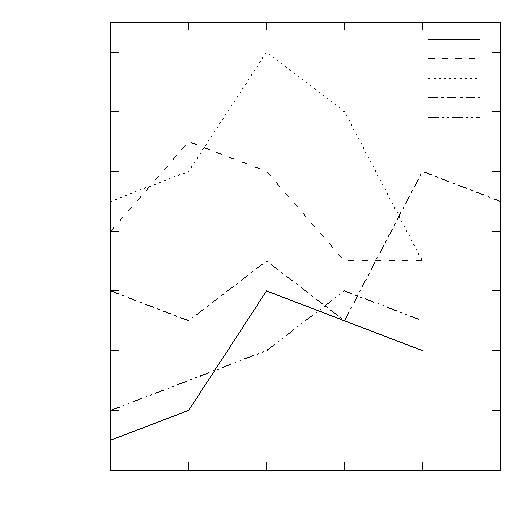
\includegraphics{mcs}}%
    \gplfronttext
  \end{picture}%
\endgroup

	\caption{Most Common Stride Threshold and Aggressiveness}
	\label{fig:prefetcher_tweaks}
\end{figure}
